\section{Orizzonte temporale}
\begin{frame}{\secname}
    \begin{itemize}
        \item Tempo di simulazione totale: 5000s
        \begin{itemize}
            \item Tempo adeguato per raggiungere la fase stazionaria in tutti i casi
            \item Tempo di simulazione per fattibilità computazionale
        \end{itemize}
        \item Fase di warm-up: 500s
        \begin{itemize}
            \item Esclusa la parte iniziale per evitare l'influenza del transitorio
            \item Alternativa possibile: 1500s
        \end{itemize}
    \end{itemize}
    \begin{center}
        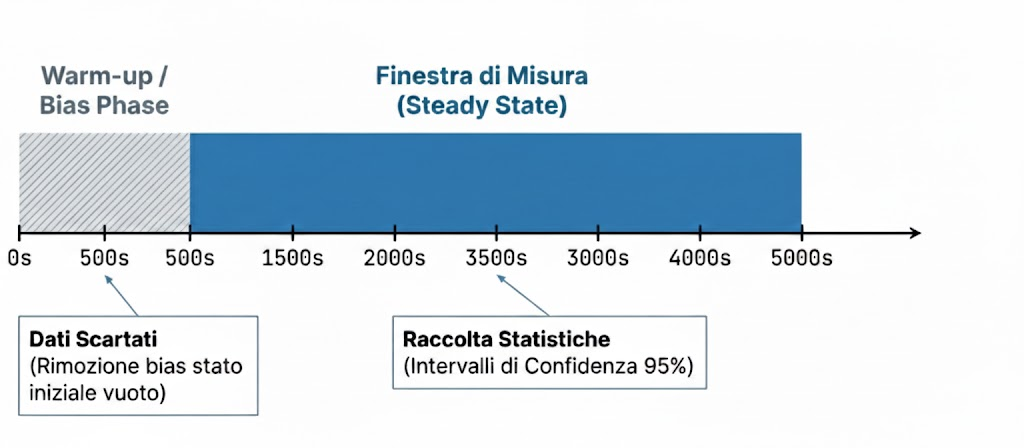
\includegraphics[width=0.8\textwidth]{../images/Orizzonte.jpg}
    \end{center}
\end{frame}